\documentclass[a4paper, 11pt]{article}
\usepackage{graphicx}
\usepackage{amsmath}
\usepackage[pdftex]{hyperref}
\usepackage{graphicx}
\usepackage[export]{adjustbox}
\usepackage{subcaption}
\usepackage{wrapfig}

% Lengths and indenting
\setlength{\textwidth}{16.5cm}
\setlength{\marginparwidth}{1.5cm}
\setlength{\parindent}{0cm}
\setlength{\parskip}{0.15cm}
\setlength{\textheight}{24cm}
\setlength{\oddsidemargin}{0cm}
\setlength{\evensidemargin}{\oddsidemargin}
\setlength{\topmargin}{0cm}
\setlength{\headheight}{0cm}
\setlength{\headsep}{0cm}

\renewcommand{\familydefault}{\sfdefault}

\title{Introduction to Learning and Intelligent Systems - Spring 2015}
\author{jo@student.ethz.ch\\ sakhadov@student.ethz.ch\\  stegeran@student.ethz.ch\\}
\date{\today}

\begin{document}
\maketitle
\section*{Project 1 : Regression}

In our project for passenger number prediction we use Linear Regression.

The most important step is feature engineering. We use the method transformFeatures for this.

We noticed from the data distribution that the Y values depend greatly on hours data features. It should not be a big surprise as the data presented are passenger numbers.
Figure 1 shows this dependency.

\begin{figure}[h]
 
\begin{subfigure}[l]{0.5\textwidth}
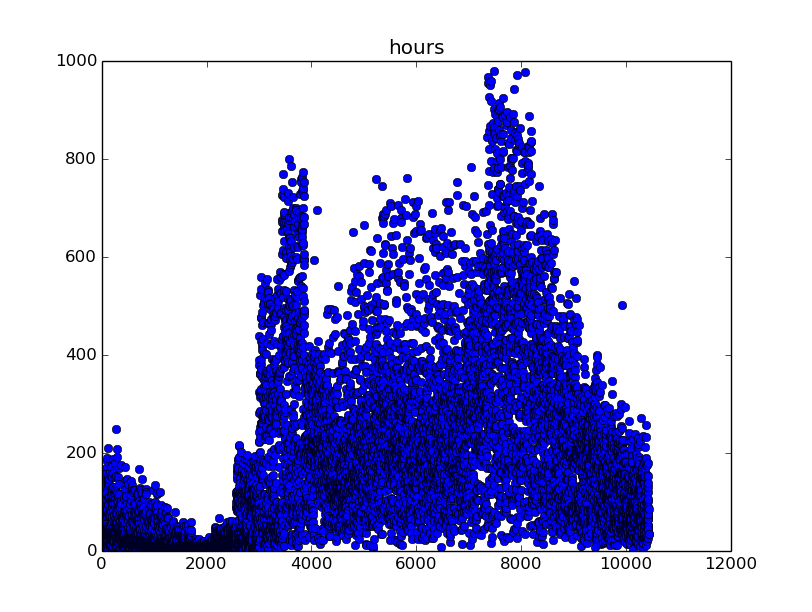
\includegraphics[width=0.9\linewidth, height=5cm]{Plots/hours} 
\caption{Given data}
\label{fig:subim1}
\end{subfigure}
\begin{subfigure}[r]{0.5\textwidth}
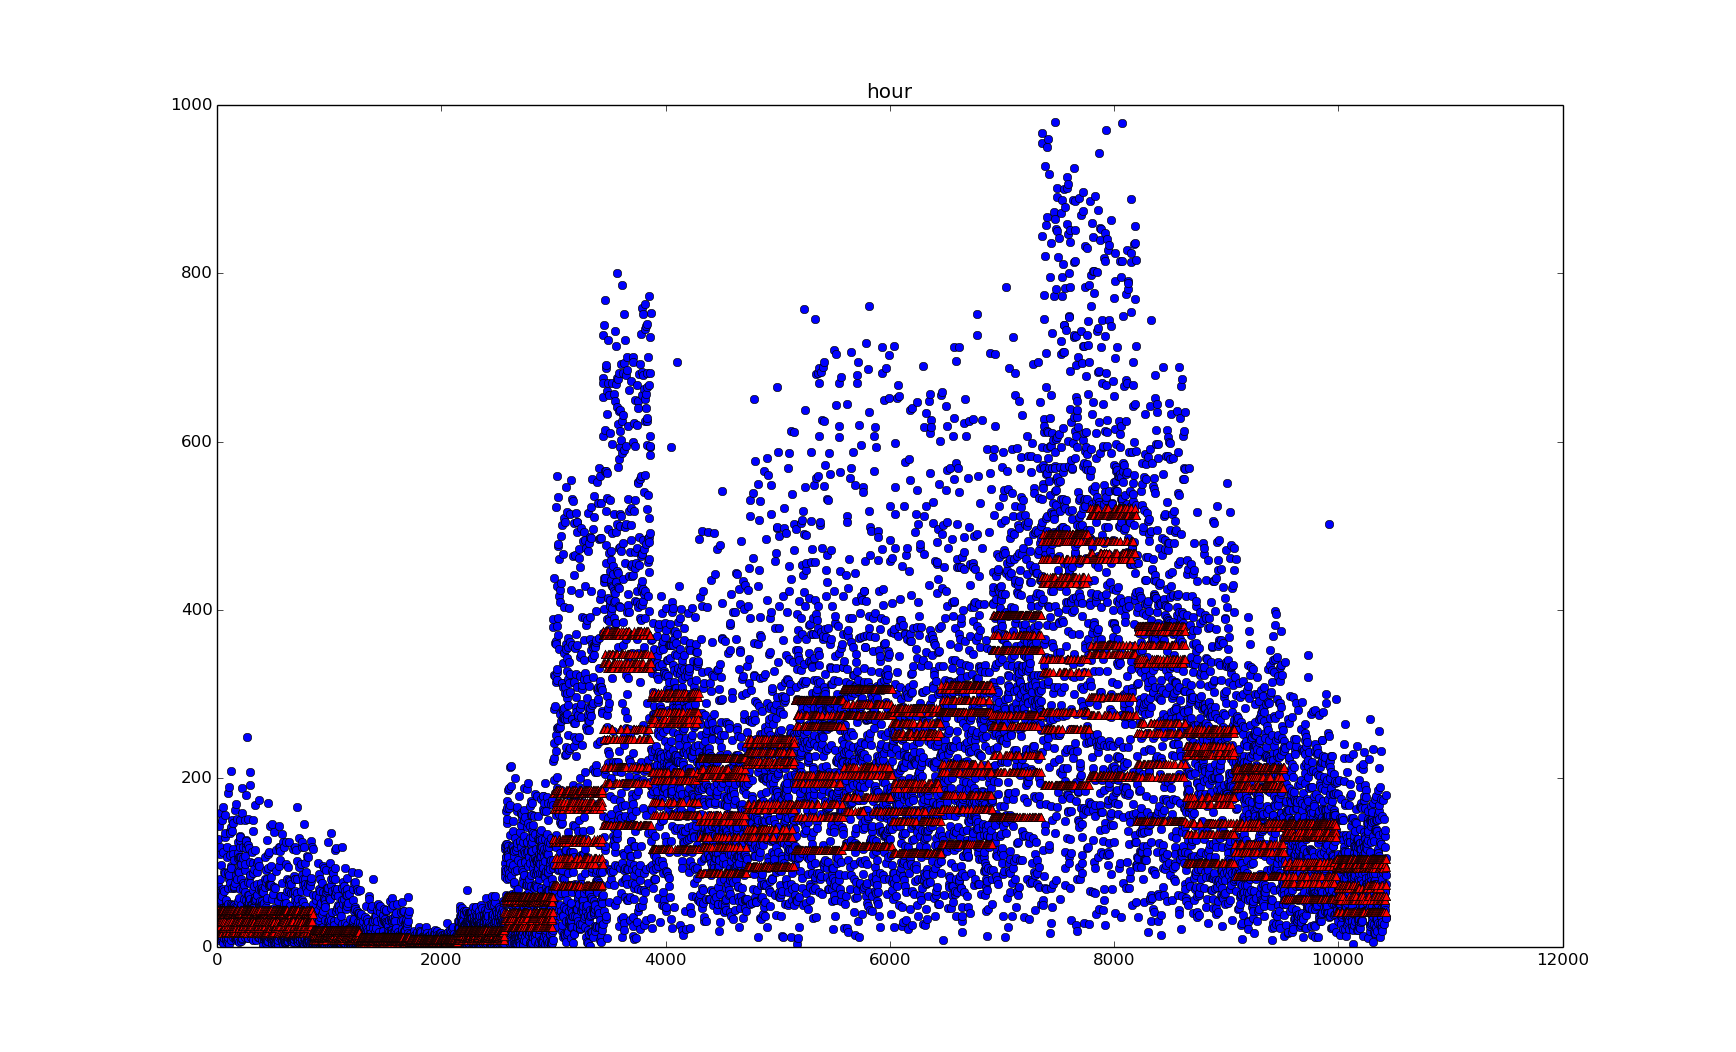
\includegraphics[width=0.9\linewidth, height=5cm]{Plots/hours_predicted}
\caption{Our resulting prediction}
\label{fig:subim2}
\end{subfigure}
 
\caption{Y values sorted by hour}
\label{fig:image2}
\end{figure}

Additionally we use other features such as month, year, day of year and the factors A-F.


\begin{wrapfigure}{r}{0.4\textwidth}
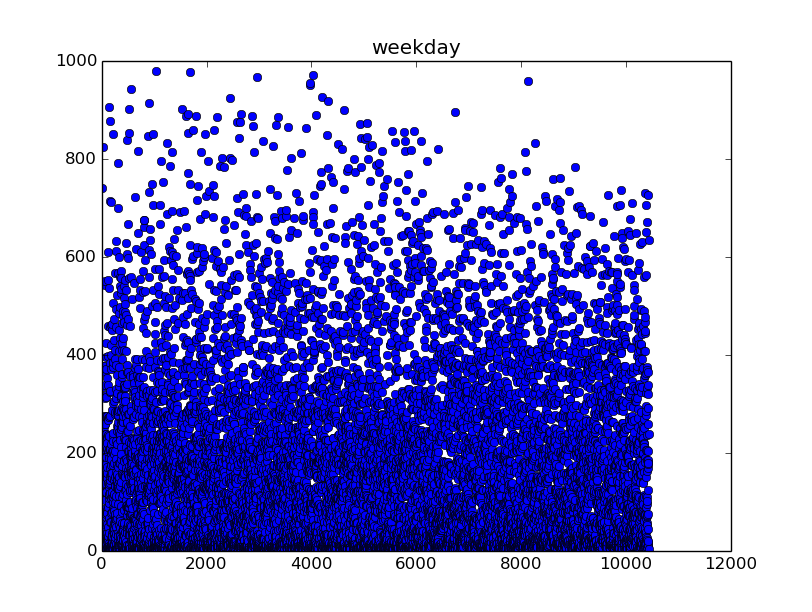
\includegraphics[width=0.9\linewidth]{Plots/weekdays} 
\caption{Y values sorted by weekdays}
\end{wrapfigure} We construct our feature vectors for hour values with monomials of the degree up to 5. Combining hour values and minutes did not give any score gain.

The weekdays were divided in two bins. The working days and the weekend. The working days had generally more passengers during the day than the weekends as the Figure 2 shows. We also noticed that half of the data was on the weekends. We tried to use this knowledge and weight the data points on the working days higher. However this approach did not produce any substantial results. 
\clearpage

\begin{wrapfigure}{r}{0.4\textwidth}
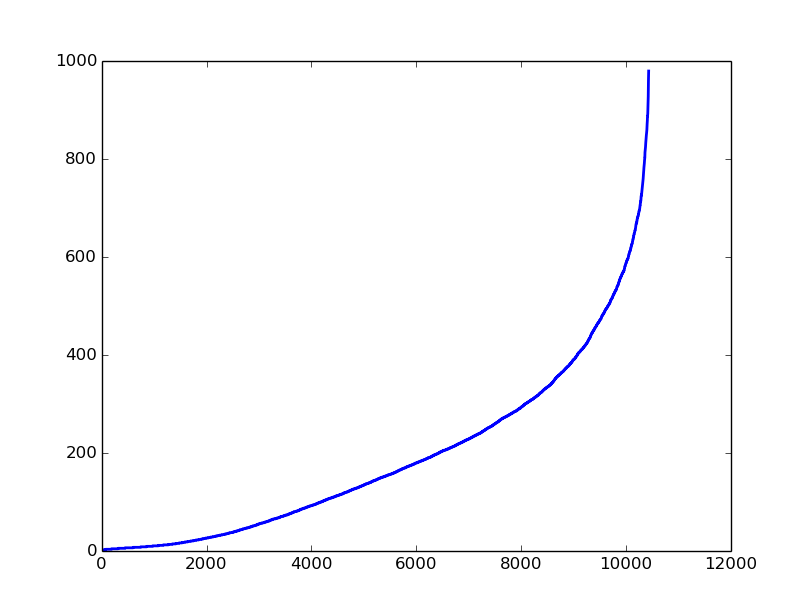
\includegraphics[width=0.9\linewidth]{Plots/data_sorted} 
\caption{Y data sorted by value}
\end{wrapfigure}
 
Other important point to make is that the data is roughly exponentially distributed. This can be seen on the Figure 3. For the fitting we took therefore the logarithm of the values. This allowed for better linear regression and considerable predication accuracy gain. The predicted values had then to be transformed back with exponential function in order to get the actual approximation. This step also takes care of the negative values.

Combing features together we achieved further improvement. To capture the correlation between hours and other factors we produced several feature vectors consisting of the products of hour vector and other features. These vectors were also expanded to monomials of the degree up to 5. 

The last step was to normalize the feature vectors. This was done per feature vector by subtracting the mean and dividing by the standard deviation.

For our regression several loss functions have been tried.
Ridge Regression and Lasso Regression both performed the same as the Linear Regression. Grid search for best coefficient alpha gave zero as the best alpha value. 
\end{document}
